\chapter{Supersimetría} %% y su fenomenología} %%Contexto Te\'orico}

\newcommand{\GM}{gauge mediation}

%% \todo[inline]{Add chapter introduction}

%% Supersimetría (SUSY) \cite{Miyazawa:1966,Ramond:1971gb,Golfand:1971iw,Neveu:1971rx,Neveu:1971iv,%
%%   Gervais:1971ji,Volkov:1973ix,Wess:1973kz,Wess:1974tw}
%% es uno de los candidatos teoricos mejores motivados para fisica mas alla del Modelo Estandar.
%% Si las particulas supersimetricas que interactuan fuertemente, es decir squarks y gluinos, estan
%% presentes a la scala del \tev, estas deberian haber sido producidas en el LHC incluso a 7 \tev.

%%

% Motivacion (From arxiv 9709356: A susy primer Introduction)
%% The SM of high energy physics, augmneted by neutrino masses, provides a remarkably succesful description of presently known phenomena. The experimental frontier has advance into the
%% TeV range with no uambiguous hints of additinal structure. Still, it seems clear that the SM is a work in progress and will have to be extended to describe physcis at higher energies. Certainly,
%% a new framework will be required at the reduced Planck scale $M_P =  (8\pi G_\text{Newton})^{-1/2} = 2.4 \times 10^{18} \gev$, where quatum gravitational effects become important. Based only
%% on a proper respect for the power of Nature to surprise us, it seems nearly as obvious that new physcis exists in the 16 order of magnitude in eenrgy between the presently explored territory near the electroweak scale,
%% $M_W$, and the Planck scale. ...

%%\section{Motivaci\'on}
%% \itodo{Tener en cuenta que el capitulo anterior termina contando las debilidades de ME y mostrando
%%   las alternativas para fisica mas alla del ME}

\section{Supersimetría}

El Modelo Est\'andar de la f\'isica de altas energ\'ias descripto en el capitulo anterior,
con el agregado de la masa de los neutrinos, y el descubrimiento del bos\'on de Higgs,
ha tenido un gran \'exito en la correcta descripci\'on de los fenómenos conocidos hasta la escala
del {\tev} que los experimentos han llegado en los utltimos a\~nos.
%% A pesar de esto, resulta claro que el Modelo Est\'andar no es una teoria definitiva y va a tener que
%% ser extendida para describir la f\'isica de altas energ\'ias.

A pesar de esto, no hay dudas respecto a que una nueva teor\'ia va a ser necesaria a la escala
reducida de Planck $M_P =  (8\pi G_\text{Newton})^{-1/2} = 2.4 \times 10^{18} \gev$ , donde los efectos
cu\'anticos gravitacionales son importantes. Es bastante claro que tiene que existir nueva f\'isica en
los 16 ordenes de magnitud en energ\'ia entre el territorio explorado cerca de la escala electrod\'ebil y
la escala de Planck.

El s\'olo hecho de que la relación $M_P/M_W$ es tan grande es una gran pista para la física mas
allá del {\SM}, por el llamado \emph{problema de jerarquía}. Aunque esta  no es una dificultad
intrínseca del {\SM},  sino ...
%% but rather a disturbing sensitivity of the Higgs
%% potential to new physics in almost any imaginable extension of the Standard Model.

La parte electricamente neutral del campo de Higgs del Modelo Est\'andar es un escalar complejo $H$ con
un potencial clasico $V=m_H^2 |H|^2 + \lambda|H|^4$.

El {\SM} necesita un valor de expectaci\'on del vacio (VEV) para $H$ en el m\'inimo del potencial no nulo.
Esto ocurre si $\lambda>0$ y $m_H^2<0$, resultando en $\langle H \rangle = \sqrt{-m_H^2/2\lambda}$.
Como experimentalmente sabemos que $\langle H \rangle$ es aproximadamente 174 \gev, de las medidas
de las propiedades de las interacciones debiles, el valor de  $m_H^2$ debe ser del orden de $-(100 \gev)^2$.

El problema es que $m_H^2$ recibe grandes correcciones cuanticas de los efectos virtuales de cada
particula a la cual se acopla, directa o indirectamente, al campo de Higgs.

\begin{figure}[h]
  \centering

  \begin{tikzpicture}[node distance=1cm and 1 cm]

  \coordinate[vertex, label=above:$H$] (v1);
  \coordinate[vertex, right=of v1] (v2);
  \coordinate[vertex, right=of v2] (v3);
  \coordinate[vertex, right=of v3] (v4);

  \draw[higgs] (v1) -- (v2);
  \draw[higgs] (v3) -- (v4);

  \draw[fermion] (1.5, 0) circle (0.5);
  \node at (1.5, 0.75) {$f$};

\end{tikzpicture}


  \caption{Correciones cu\'anticas a un loop al cuadrado de la masa del Higgs $m_H^2$ debido a la
    masa de un fermi\'on de Dirac $f$.}\label{fig:higgs_correction_f}
\end{figure}

Por ejemplo, en la {\fig} \ref{fig:higgs_correction_f} tenemos una correci\'on a $m_H^2$ del loop
que contiene un fermi\'on de Dirac $f$ con masa $m_f$. Si el campo de Higgs se acopla a $f$ con un
término en el lagrangiano igual a $-\lambda_f H \bar{f}f$, el diagrama de Feynman en la
{\fig} \ref{fig:higgs_correction_f} genera una correci\'on:

\begin{equation}
  \Delta m_H^2 = -\frac{|\lambda_f|^2}{8\pi^2} \Lambda^2_\text{UV} + \ldots
  \label{eq:higgs_corr_f}
\end{equation}
%
donde $\Lambda_\text{UV}$ es el corte ultravioleta usado para regular la integral en el \emph{loop}.
Debe ser interpretado como la m\'inima escala de energ\'ia a la cual entra la nueva física para
alterar el comportantamiento de la teoría a altas energías. Los puntos suspensivos representan
terminos proporcionales a $m_f^2$, que crecen a lo sumo logaritmicamente con $\Lambda_\text{UV}$.
Cualquiera de los leptones o quarks del {\SM} puede jugar el rol de $f$ (para el caso de quarks
la correcci\'on tiene que ser multiplicada por 3 para tener en cuenta el color).
La correci\'on m\'as grande va a ser cuando $f$ es el quark \emph{top} con $\lambda_f \approx 1$.

El problema es que si $\Lambda_\text{UV}$ es del orden de $M_P$, la correci\'on a $m_H^2$ es
30 ordenes de magnitud mas grande que el valor requerido de $m_H^2 \sim (100 \gev)^2$.
Este es solo un problema para las correcciones al cuadrado de la masa del bos\'on de Higgs escalar,
porque las correcciones cuanticas a las masas de los fermiones y los bosones de gauge no tienen una sensibilidad
cuadratica directa a $\Lambda_\text{UV}$ como la que estan en la {\eq} \eqref{eq:higgs_corr_f}. Sin embargo, los quarks, leptones
y los bosones de gauge electrodebiles $Z^0$, $W^{\pm}$ del {\SM}, todos obtienen masa de $\avg{H}$, por lo
tanto el espectro completo de masas del {\SM} es directa o indirectamnte sensible a la escala de corte
$\Lambda_\text{UV}$.

Uno puede pensar que la soluci\'on es elegir un $\Lambda$ no demasiado grande \todo{...}.

\begin{figure}[h]

  \centering

  \begin{tikzpicture}[node distance=1cm and 1 cm]

  \coordinate[vertex, label=above:$H$] (v1);
  \coordinate[vertex, right=of v1] (v2);
  \coordinate[vertex, right=of v2] (v3);
  \coordinate[vertex, right=of v3] (v4);

  \draw[higgs] (v1) -- (v2);
  \draw[higgs] (v2) -- (v3);
  \draw[higgs] (v3) -- (v4);

  \draw[higgs] (1.5, 0.5) circle (0.5);

  \node at (1.5, 1.25) {$S$};

\end{tikzpicture}


  \caption{Correciones cu\'anticas a un loop al cuadrado de la masa del Higgs $m_H^2$ debido a la
    masa de un escalar $S$.}\label{fig:higgs_correction_s}
\end{figure}

En el caso de que exista un escalar complejo pesado $S$ con masa $m_S$ que se acopla al Higgs con un
termino en el Lagrangiano $-\lambda_S \abs{H}^2 \abs{S}^2$, el diagrama de Feynman es el que se muestra
en la {\fig} \ref{fig:higgs_correction_s} y este da lugar a una correcci\'on:

\begin{equation}
  \Delta m_H^2 = \frac{\lambda_S^2}{16\pi^2} \left[ \Lambda^2_\text{UV} - 2 m_S^2 \ln (\Lambda^2_\text{UV}/m_S) +  \ldots \right]
\end{equation}

%% Puede ser que el boson de Higgs no sea una fundamenta, como en modelos technicolor, o modelos en
%% los cuales el Higgs es compuesto.
Si el bosón de Higgs es una partícula fundamental y hay física a una escala mucho mayor a la
escala electrodo, existen dos opciones: tenemos que hacer alguna asumpcion bizarra que no existe ninguna
partícula de mayor masa o efectos que se acoplen (incluso indirectamente o extremadamente débiles) con el
campo escalar de Higgs, o algún tipo de  cancelación es necesaria entre las varias contribuciones a $\Delta m_H^2$.


Afortunadamente la cancelaci\'on de todas estas contribuciones a las masas escalares no solo es posible,
sino que es inevitable, si consideramos que existe una simetría que relaciona fermiones y bosones.
A esta simetria la llamamos supersimetría (SUSY).
Una transformación supersimétrica convierte un estado bosónico en uno fermiónico, y viceversa.
El operador $Q$ que genera estas transformaciones debe ser un spinor anticonmutativo, con

\begin{equation}
  Q \ket{\text{bos\'on}} = \ket{\text{fermi\'on}}, \quad \quad Q \ket{\text{fermi\'on}} = \ket{\text{bos\'on}}
\end{equation}

Los espinores son intrínsecamente objectos complejos, por lo tanto el conjugado hermitico de $Q$ es también
un generador de la simetría. Debido a que $Q$ y $Q^\dagger$ son operadores fermiónicos,
llevan momento angular de spin 1/2, por lo tanto es claro que susy debe ser una simetria espacio-temporal.

En una extensión superimétrica del {\SM}, cada una de las part\'iculas fundamentales conocidas esta en un supermultiplete
quiral o de gauge, y debe tener una super-compa\~nera con spin que difiere en $1/2$.
Los nombres de de las super compa\~neras de spin 0 de los quarks y leptones son construidos agregando
una ``s'' (de escalar) al nombre: squarks y sleptones.

Los supermultipletes quirales y de gauge de las tablas conforman el contenido de partículas del Modelo
Estándar Supersimétrico Mínimo (MSSM). Una característica interesante de esta teoría es que ninguna
de las compa\~neras supersimétricas de las partículas del {\SM} han sido observadas hasta el momento.
Si SUSY no estuviera rota, deberían existir selectrones con una masa igual a $m_e \sim 0.511 \mev$,
y lo mismo para los demás sleptones y squarks. Y también deberían existir los
gluinos y fotinos sin masa. De ser asi, estos deberían haber sido descubiertas tiempo atrás. El hecho
de que no haya sido asi es motivo evidente que la supersimetría es una simetría que esta rota en el
estado de vacío elegido por la naturaleza.

El problema es que el hecho de que la supersimetría no este rota es lo que garantizaba que las
divergencias cuadráticas en el cuadrado de las masas escalares debían anularse a todo orden en
teoría de perturbaciones.
Para que SUSY todavía provea la solución al problema de jerarquía incluso en presencia del rompimiento
de esta, las relaciones entre los acoplamientos adimensionales que están en la teoría
no rota deben mantenerse. %De otra forma, van a existir correcciones radiativas cuadráticas divergentes
%a las masas escalares del Higgs de la forma

Por lo tanto el rompimiento de la simetría debe ser \emph{soft}. El Lagrangiano efectivo del MSSM tiene
que poder ser escrito

\begin{equation}
  \mathcal{L} = \mathcal{L}_\text{SUSY} + \mathcal{L}_\text{soft}
\end{equation}
%
donde $\mathcal{L}_\text{SUSY}$ contiene todas las interacciones de gauge y de Yukawa y preserva la
invarianza supersimétricas, y $\mathcal{L}_\text{soft}$ viola supersimetría pero contiene solo
términos de masa y parámetros de acoplamientos con dimensión de masa positiva.
Si la escala de masa mas grande asociada  con los términos soft se llama $m_\text{soft}$, las
correcciones adicionales no supersimétricas al cuadrado de la masa escalar del Higgs debe anularse en
el limite $m_\text{soft} \to 0$.

Debido a la diferencia de masas entre las partículas conocidas del SM y sus súper-compañeras son
determinadas por los parámetros $m_\text{soft}$ que aparecen en $\mathcal{L}_\text{soft}$, las masas
de las partículas supersimétricas no pueden ser demasiado grandes. De otra forma perderíamos la
solución al problema de jerarquía.

Existe una razón por la cual las partículas supersimétricas deben ser lo suficientemente pesadas para
no haber sido descubiertas. Todas las demás partículas del MSSM que han sido descubiertas tienen algo
en com\'un: deberían no tener masa en ausencia del rompimiento de la simetría electrodébil. En
particular, las masas de los bosones $W^\pm$, $Z^0$ y todos los quarks y leptones son iguales a constantes
de acoplamenitneo adimensionales por el Higgs VEV $\sim 174 \gev$, mientras que el fotón y el gluon
necesitan ser no masivos por la invarianza de gauge electromagnética y de QCD. Y por el contrario,
todas las partículas del MSSM no descubiertas tienen la propiedad contraria. Cada una de ellas pueden
tener un término de masa en el Lagrangiano en ausencia del rompimiento de simetría electrodébil.

Una característica importante del MSSM es que las súper-compañeras listadas en la tabla no son
necesariamente autoestados de masa de la teoría. Esto es porque después del rompimiento de la simetría
electrodébil y SUSY, puede haber mezcla entre los gauginos y higgsinos, y entre los squarks y sleptones
y los Higgs escalares que tienen la misma carga eléctrica. La única excepción es el gluino.

Las masas y las mezclas de las súper partículas son de extrema importancia desde el punto de vista
experimental. Y estos problemas fenomenológicos están relacionados con una cuestión central:
De que forma SUSY esta rota?


%------
% MSSM
%------
\section{Modelo Mínimo Estándar Supersimétrico}

La extension del {\SM} que requiere la introduccion de la minima cantidad de particulas es llamado
MSSM. Los terminos de masa son agregados al Lagrangiano

Dada la naturaleza de los campos quirales introducidos en la implementacion de SUSY, solo el campo
escalar de Higgs no es suficinete para dar masa a los fermiones izquierods y derechos. Se debe
agregar un nuevo campo escalar para compensar. En el ME, el campo de Higgs es un doblete, y de los
cuatro graods de libertad solo uno permanece como consecuencia del rompimiento de la simetria EW, resultando
en un boson de Higgs. Los dos dobletes de Higgs del MSSM son:
%
\begin{equation}
  H_u = \binom{H_u^+}{H_u^0}, \quad \quad \quad H_d = \binom{H_d^0}{H_d^-}
\end{equation}
%
con un total de 8 grados de libertad, 3 de los cuales se pierden en el rompimiento EW. Por lo que
quedan 5 bosones de  Higgs en el MSSM: $h^0, H^0, H^+, H^-, A^0$. El mas liviano de los 5 es $h^0$
el cual es el mas similar al del ME.

En el ME, la mezcla de los bosones de guage electrodebiles dan lugar los autoestados de masa \gam, Z y $W^\pm$.
En el MSSM los higgsinos neutros y los gauginos se mezclan para formar los cuatro neutralinos:
\ninoone, \ninotwo, \ninothree\ y \ninofour.
Y de forma similar los higgsinos cargados y los winos dan lugar a los dos charginos, \chinoonepm\ y \chinotwopm.



En el MSSM se agrega una nueva simetrai, que tiene como objetivo.... Esta nueva simetria se conoce
como paridad-R

\begin{equation}
  P_R = (-1)^{3(B-L)+ 2s}
\end{equation}

Las partículas con paridad-R impar se llaman partículas supersimétricas o ``sparitculas''.

Si la paridad-R es exactamente conservada, no puede haber mezcla entre las sparituclas y las
particulas con $P_R = +1$. Cada vertice de interaccion en la teoria contine un numer par de
sparticulas. Esto tiene tres consecuencias fenomenologicas de extrema importancia:

\begin{itemize}
\item La part\'icula supersimetrica mas liviana, llamada LSP, debe ser estable. Si la LSP es
  electricamente neutra, interactua solo de forma d\'ebil con la materia ordinaria, y por lo tanto
  resulta en un candidato muy atractico para la materia oscura no barionica que es requerida por
  la cosmolog\'ia.
\item Cada part\'icula supersimetrica que no sea la LSP debe decaer eventualmente en un estado que
  contenga un numero impar de LSPs (en general una).
\item En experimentos de colisionadores, las particulas supersimetricas pueden solo ser producidas
  en numero par, en general de a dos.
\end{itemize}


Se suele definir al  MSSM


%% % From Emma
%% Supersimetria (SUSY) postula una nueva simetria entre fermiones y bosones tal que cada particula
%% del ME tiene su super-compa\~nera cuyo spin difiere en 1/2. Estas particulas supersimetricas
%% deberia ser identica a sus compa\~neras del ME, excepto en el spin. La convecion para sus nombres
%% is agregar una ``s'' como prefijo para las compa\~neras de los fermiones y el sufijo ``-ino'' para
%% las super-compa\~neras de los bosones...

%% Si SUSY representa una simetria exacta entre fermiones y bosones, las particulas supersimetricas
%% deberias tener la misma masa que sus companeras del ME.






\begin{tikzpicture}



\end{tikzpicture}


%---------------------
% Rompimiento de SUSY
%---------------------
%% \section{Origen del rompimiento de la Supersimetr\'ia}

%% Existen dos principales propuestas que compiten por cuales deben ser las ineracciones mediadoras



%% \begin{figure}[h]
%%   \centering

%%   \begin{tikzpicture}

%%     \draw (0,0) rectangle (4,2);
%%     \draw (6,0) rectangle (10,2);

%%     \node at (3.9,1) (r1) {};
%%     \node at (6.1,1) (r2) {};

%%     \draw[decorate,decoration={snake}] (r1) -- (r2);

%%   \end{tikzpicture}

%% \end{figure}

%------
% GMSB
%------
\section{Modelos de rompimiento de supersimetria mediados por campos de Gauge}

%% \itodo{Check General Gauge Mediation. Meade, Seiberg, Shih}

En los modelos de rompimiento de la supersimetria mediado por campos de gauge (GMSB), las
interacciones ordinarias de gauge son los responsables de la aparicion
del rompimiento de la supersimetria ``soft'' en el MSSM. La idea basica es introducir neuvos
supermultipletes quirales, llamados mensajeros, que se acoplen ...


\section{El espectro de masas del MSSM}

\subsection{Neutralinos}
Los higgsinos y los gauginos electrodebiles se mezclan entre ellos debido al efecto del rompimeinto
de la simetria electrodebil. Los higgsinos neutros ($\susy{H_u^0}$ y $\susy{H_d^0}$) y los
gauginos neutros (\bino, \winozero) se combinan para formar cuatro autoestados de masa llamados
neutralinos. Los higgsinos cargados ($\susy{H_u^+}$ y $\susy{H_d^-}$) y los winos
(\winop y \winom) se mezclan para formar dos autoestados de masa con carga $\pm 1$ llamados
charginos. A continuacion se utilizara la siguiente notacion para llamar a los neutralinos y charginos:
${\nino}_{i}$ ($i=1,2,3,4$) y ${\chinopm}_{i}$ ($i=1,2$) donde estos son ordenados de forma ascendente segun su
masa. El neutralino mas liviano {\ninoone}, suele ser la LSP, salvo que exista un {\gravino} mas
liviano o que la paridad-R no se conserve.

En la base de autoestados de gauge $\psi^0 = (\bino, \winozero, \susy{H_d^0}, \susy{H_u^0})$,
la parte de masa del neutralino del Lagrangiano es

\begin{equation}
  \mathcal{L}_\text{neutralino mass} = -\frac{1}{2} (\psi^0)^T M_{\nino} \psi^0 + c.c.
\end{equation}

donde

\begin{equation}
  M_{\nino} = \left(
  \begin{array}{cccc}
    \M{1} & 0 & -c_\beta s_W m_Z &  s_\beta s_W m_Z \\
    0 & \M{2} & c_\beta c_W m_Z & -s_\beta c_W m_Z \\

    -c_\beta s_W m_Z & c_\beta c_W m_Z & 0 & -\mu \\
    s_\beta s_W m_Z & -s_\beta c_W m_Z & -\mu & 0 \\
  \end{array}
  \right)
\end{equation}

Esta matriz de masas puede ser diagonalizada con una matriz unitaria N para obetener los autoestados
de masa:

\begin{equation}
  \nino_i = N_{ij} \psi^0_j
\end{equation}

%% tal que

%% \begin{equation}
%%   N^{*} M_{\nino} N_{-1} =  \left(
%%   \begin{array}{cccc}
%%     m_{\ninoone} & 0 & 0 & 0 \\
%%     0 & m_{\ninotwo} & 0 & 0 \\
%%     0 & 0 & m_{\ninothree} & 0 \\
%%     0 & 0 & 0 & m_{\ninofour}
%%   \end{array}
%%   \right)
%% \end{equation}


Los autoestados de masas y la matriz de mezcla $N_{ij}$ pueden obtenerse en termino de los parametros
\M{1}, \M{2}, $\mu$ y $\tan\beta$.

El sector de los neutralinos esta determinado por tres parametros reales, \M{1}, $\tan\beta$ y
$\mu$ (como tambien por supuesto $m_Z$ y $\theta_W$).


\subsection{Charginos}

Los analogos cargados de los neutralinos son los charginos

\subsection{Gluinos}

Como el gluino es un \fix{colour octet fermion}, no puede mezclarse con ninguna
otra particula del MSSM, incluso si la paridad-R es violada. La mayoria de los
modelos asumen que la masa del gluino es significativamente mayor  que los
neutralinos y charginos.





\section{Fenomenologia del GGM}

\itodo{arxiv 9601367}

\begin{equation*}
  m_{\gravino} = \frac{F}{\sqrt{3} M_p} \sim \left( \frac{F}{(100 \tev)^2} \right) \mathrm{eV}
\end{equation*}
where F is the susy breaking scale.

The lightest standard model supersymmetric
particle is then the NLSP, and can decay to its partner and the
gravitino.
The decay to the Goldstino component is then suppressed
only by F rather than Mp. In the case that the NLSP is mostly bino, the
coupling leads to a transition magnetic dipole moment between the NLSP
and gravitino, $\cos\theta_W (m_{\bino}/2\sqrt(2) F) \bino \bar{\sigma}^\mu \sigma^\nu F_{\mu\nu} + h.c.$,
giving rise to a decay rate

\begin{equation*}
  \Gamma(\bino\to \gravino + \gamma) = \frac{\cos^2\theta_W m_{\bino}^5}{16\pi F^2}
\end{equation*}

This translates to a decay length

\begin{equation}
  c\tau \approx 130 \left( \frac{100 \gev}{m_{\bino}} \right)^5 \left( \frac{\sqrt{F}}{100 \tev} \right)^4 \mu m
\end{equation}
So there is a range of F and m for which the decay occurs within the detector, with the gravitino carrying off missing energy. For$ mB > mZ$ there is
also a non negligible branching fraction $B\to\gravino + Z$

Depending on the specific decay modes of the nlsp, displaced vertices for $\sqrt{F}$ between roughly 100-1000 of \tev could be accessible to collide experiments.

This range of experimentally accessible $\sqrt{F}$ is in fact consistent with strophysical and cosmological considerations. Unless there is an inflation with low
reheat temperature, avoiding overclosure of the universe from relic gravitinos requires $\sqrt{F} \sim \leq 2 \times 10^3 \tev$






arxiv 9801254

Fine tuning arguments suggest that the SUSY masses should be below about 1 TeV if SUSY is relevant to electroweak physiscs.
Then SUSY production at the LHC is dominated by the production of gluino and squarks.

arxiv 1103.6083

%% Gauge mediation is an extremely well-motivated and theoretically-sound supersimmetric scenario. It autmatically solves the SUSY flavor
%% problem, and it provides a calculable and predictive framework. It also has rich and distinctive phenomenology.

En gauge mediation, la LSP es el gravitino, que es muy liviano. Por lo tanto la partícula mas liviana
del MSSM es la NLSP, que siempre decae en un gravitino y su super-compa\~nero del {\SM}. Como este
decaimiento está fuertemente suprimido por la escala de rompimiento de SUSY, el decaimiento de la NLSP
puede ser \fix{prompt} o desplazado. Esta supresión de la taza de decaimiento también significa que todas las
partículas supersimétricas mas pesadas decaen primero en la NLSP antes de decaer en el gravitino. Por lo
tanto la naturaleza de la NLSP es el aspecto más importante del espectro de los modelos GMSB en las signatures
de los colisionadores.

\itodo{La NLSP puede ser cualquier .... Focus on neutralino NLSP}

\subsection{General Neutralino NLSP}

En el caso de que la NLSP sea el neutralino, la fenomenolog\'ia se puede entender mejor yendo a
algunos limites simplificados de los autoestados. De esta forma los distintos tipos son:

\begin{itemize}
\item bino NLSP
\item wino co-NLSP
\item higgsino NLSP
\end{itemize}

%% We will formulate minimal spectra in this paper which allow for significant strong SUSY production at the early LHC,
%% and populate the many final states   available to general neutralino NLSPs.

El espacio de parametros consiste esencialmente en una scala de produccion de color (masa del gluino)
y la masa de la NLSP. Todas las demas sparticulas se desacoplan que no son esecnailes en la producción
de la signatur de interes. De alguna forma, esto es similar a utilizar ``modelos simplifciados'' como
se utilizan en muchos estudios fenomenoligicos y experimentales. \todo{add references?}


El neutralino NLSP decae a $X + \gravino$, donde $X=\gamma, Z, h$, y los diferentes autoestados de gauge
se caracterizan por tener distintos branching fractiones a las diferentes $X$.

  %% The branching fractions of the bino-like and wino-like neutralino NLSP are shown in the figure.
  %% \includegraphics[width=0.5\textwidth]{br_bino}
  %% \includegraphics[width=0.5\textwidth]{br_wino}

Los binos decaen a fotones con un BR $\sim \cos^2\theta_W$, con una componente menor a Z's, con
BR $\sim \sin^2\theta_W$.
Por otro lado estos BR se intercambian en el caso de que la NLSP sea el wino neutro, que decae
mayormente a Z's.
Si la NLSP es higgsino, este decae en forma dominante a Z o $h$, con branching ratio que depende
en el valor de $\tan\beta$ y del signo de $\mu$. Hay tres casos:

\begin{itemize}
\item El decaimiento del higgsino es dominantemente a Z a bajo $\tan\beta$ y $\mu$ positivo,
\item rico en $h$ a bajo $\tan\beta$ y $\mu$ negativo,
\item y una mezcla de $Z$ y $h$ a moderado y alto $\tan\beta$.
\end{itemize}

Cuando la NLSP es mayormente wino, hay una muy pequena degeneracion entre el wino neutro y el
cargado\todo{ref 42}. Cuando esto pasa, el decaimiento de tres cuerpos al wino neutro comienza
a ser excluido, y el wino cargado prefiere decaer directamente a $W^{\pm}$ y un gravitino \todo{ref 11}.
En otras palabras, el wino neutro y el wino cargado se vuelve co-NLSPs, y los estados finales van
a contener $W$'s, $Z$'s y fotones.

Por otro lado, la degenraci\'on entre los higgsinos cargados y neutros es generalmente mayor, de modo
que solo el neutralino mas livinao decae directamente en gravitino.

El espectro simplificado se muestra en la figura. Basicamente consideramos variar la masa del gluino
(\M{3}) y la masa de la NLSP (\M{1}, \M{2} ó $\mu$ dependiendo si la NLSP es bino, wino ó higgsino,
respectivamente). Todos los demás estados están desacoplados (sus masas seteadas a 2.5 \tev), ya que
no juegan un rol importante en las signautres que nos interesan.

\includegraphics[width=0.5\textwidth]{figures/figura} %simplified_mass_spectrum}


%% We emphasize that these minimal
%% parameter spaces do correspond to physical models, since the entire GGM parameter space
%% was covered by a perturbative messenger model in [10]

%% Our simplified spectra are characterized by several types of SUSY production, with NLO
%% cross-sections shown in figure 4. For each benchmark, there is colored gluino production, with
%% rate set by the gluino mass. For the wino and higgsino NLSPs, there is also the possibility of
%% direct NLSP production with electroweak cross-sections. While the Tevatron currently has
%% the advantage here because of its much larger dataset, we will see below that the LHC will
%% have sensitivity to electroweak production with & 1 − 5 fb −1

\subsection{Bino NLSP}

The dominant decay mode for the bino NLSP is to a photon and gravtitino. The leading channel is the diphoton signature because of the large branching ratio of about $(\cos^2\theta_W)^2 \sim 0.6$,
and low SM background.

\subsection{Wino co-NLS}

\subsection{Z-rich higgsino NLSP}

Higgsinos introduce  an important difference in the topology of the gluino decays. In the bino and wino benchmarks, the gluino decayed 3-body to the neutralino and two jets,
through an off-shell squark. But the higgsino couples predominantly yo heavy flavor, where the mass of the top can squeeze out the 3-body decays. In this regime, the dominant gluino decay is
a one-loop two body decay, $\gluino\to g\susy{H}_{1,2}$.

\subsection{Other higgsino types}

The higgsino dominantly decays to Z's at low tanb and positive mu. For larger values of tanb, the higgsino decays to a roughly even mixture of Z's and h's


\section{Producción en el LHC}

\todo[inline]{add gluino production.decays diagrams, two-body, three-body}

En los colisionadores hadronicos, las sparticulas pueden ser producidas en pares a partir
de colisiones de partones de electroweak strength.

\begin{align}
  &q\bar{q} \, \to \, \chinop \chinom, \nino \nino \\
  &q\bar{q} \, \to \, \susy{\ell}^{+}_{i}\susy{\ell}^{-}_{j}, \susy{\nu}_{\ell}\susy{\nu}^{*}_{\ell}
\end{align}

y reacciones de QCD strength:

\begin{align}
  gg \qquad &\to \qquad \gluino\gluino, \susy{q_i}\susy{q_j}^{*}, \label{eq:gg}\\
  gq \qquad &\to \qquad \gluino\susy{q_i}, \label{eq:gq} \\
  q\bar{q} \qquad &\to \qquad \gluino\gluino, \susy{q_i}\susy{q_j}^{*}, \label{eq:qqbar} \\
  qq \qquad &\to \qquad \susy{q_i}\susy{q_j}, \label{eq:qq} \\
\end{align}

Las dos primeras reacciones obtienen contribuciones de los vectores bosonicos
electrodebiles en el canal $s$, y los de la primera tambien tienen contribuciones
del canal $t$ que son menos importantes en la mayoria de los modelos.
Los procesos en \eqref{eq:gg,eq:gq,eq:qqbar,eq:qq} tienen contribuciones del intercambio
del correspondiente squark o gluino en el canal $t$, y \eqref{eq:gg} y \eqref{eq:qqbar}
tambien tientn contribuciones de gluones en el canal $s$.


En Tevatron, los procesos de produccion de charginos y neutralinos tienden a tener
mayores seccion eficaz, a menos los squarks o el gluino sean muy liviano (menos a 300 \gev,
masas que ya se encuentran excluidas por el LHC). En el LHC, la situacion es opuesta, con la
produccion de gluinos y squarks dominante por medio de gluon-gluon y gluon-quark fusion.
En ambos colisionadores, puede haber produccion asociada de chargino o neutralino junto con
un squark y un gluino, pero la mayoria de los modelos predicen que la seccion eficaz




%% \section{arxiv 0911.4130}
%% SUSY breaking in the MSSM introduces ~ 100 parameters

%% Una de las caracteristicas mas caracteristica de gauge medaition es el gravitiino liviano $m_{3/2}<<M_\text{weak}$.
%% Esto asegura que los efectos de gauge mediation dominan por sobre  las contribuciones suprimidas de
%% Plank de la mediacion por gravedad. Esto implica que la la supercompanera mas liviana del MSSM es realemnte
%% la NLSP, que siempre tiene que decaer en un gravitino mas su compnera del {\SM}. El gravitino siempre
%% va a escapar del detector, dejando una gran cantidad de energia faltante. Mientras tanto , la companera
%% del {\SM} va a ser por lo general central y enrgetico (asumiendo que la NLSP decae promptly), ya
%% que es en general mucho mas liviano que la NLSP. Y dado que en cada evento se producen un par de NLSP,
%% las inclusive signautes en los colisionadores de GMSB van a ser largamente determinadas por la naturaleza
%% de la NLSP.

%% En 20\todo{Check ref 20} se estudia la cuestion de como formular gauge mediation en una forma que sea model-independent.
%% Esto resulto en el desarrollo de General Gauge Mediation (GGM), en el cual el espacio entero de los
%% posibles modelos de guage medation  pueden ser investigados sin tener que basarse en modelos especificos.

%% El conjunto completo de paramentros independientes de gauge mediation puede derivarse: tres masas
%% de gauginos complejas $M_{1,2,3}$ y tres parametros reales que controlan las masas cuadradas de
%% los 5 sfermiones $m^2_{Q,U,D,L,E}$. Tambien se ha argumentado que en el marco de GGM, los terminos
%% trilineares $A$ son siempre pequenos.

%% Cualquier spartícula del MSSM puede ser la NLSP en {\GM}. Si la NLSP es una sparticula con carga
%% de color, la signatura inclusiva (asumiendo decaimientos prompt) es dijet + \met.

%% La NLSP también puede ser un slepton, aunque es muy chica la produccion directa de sleptones en
%% el LHC, pero si pueden producirse en cascadas de decaimiento originadas en producción de pares de
%% sparticulas con color, o charginos y neutralinos. Por lo tanto las busquedas de sleptones tienen
%% que ser necesariamente mas dependientes del modelo, involucrando mas parametros del espectro.

%% Y finalmente, tenemos la posibilidad de que la NLSP sea un neutralino o chargino. Los charginos
%% s\'olo pueden ser NLSP en regiones muy peque\~nas del espacio de par\'ametros. Entonces nos queda
%% como la ultima posibilidad que la NLSP sea del tipo neutralino.

%% En general, el neutralino puede ser una mezcla arbitraria de los autoestados de gauge bino, wino
%% y higgsino. Entonces el hecho de tener un par de nuetralinos en cada evento de SUSY, da lugar a
%% signatras inclusivas involucrando combinaciones (adecuadamente elegidas) de $\gamma + \met$,
%% $Z + \met$ o $h + \met$. Una de las signaturas mas estudiadas tanto en Tevatron como el LHC ha sido
%% $\gam\gam + \met$. Adicionalmente, si la degeneracion entre las masas del neutralino NLSP y el chargino
%% mas liviano, puede haber cadenas de decaimiento que terminen con un estado final de $W^{\pm} + \met$.


%%\section{De la Nota+Paper}
%% Las teorias Gauge Mediated Symmetry Breaking (GMSB) \cite{Dine:1981gu,AlvarezGaume:1981wy,%
%%   Nappi:1982hm,Dine:1993yw, Dine:1994vc,Dine:1995ag}
%% consideran un sector oculto en el cual la supersimetria esta rota y la rotura de la simetria
%% es comunicada a los sectores visibles a traves de las interacciones de bosones de gauge del
%% modelo estandard.


%% Theories of Gauge Mediated Symmetry Breaking (GMSB)  presume a hidden sector in which supersymmetry is
%% broken and the symmetry breaking is communicated to the visible sectors through Standard Model gauge boson
%% interactions. Such theories are especially attractive because the hypothesis of an intermediate hidden sector
%% suppresses the magnitude of flavor-changing neutral currents. The lightest supersymmetric particle (LSP) in GMSB
%% is the ultra-light gravitino (\gravino), which under certain circumstances is a viable dark matter candidate \cite{Goldberg:1983nd,Ellis:1983ew}.
%% The \gravino\ has a derivative coupling to each particle and its superpartner with an interaction strength inversely
%% proportional to $\sqrt{F}$, where $F$  is a vacuum expectation value of an auxiliary field which determines the
%% magnitude of supersymmetry breaking in the vacuum state.



%% %% If the \ninoone\ is bino-like, the main decay mode is $\ninoone\to\gam\gravino$. If the \ninoone\ is
%% %% higgsino-like, it decays as $\ninoone\to h\gravino$. In addition, since the longitudinal polarisation component of the Z boson is also a Goldstone
%% %% mode of the Higgs field, a higgsino-like neutralino can also decay as $\ninoone\to Z\gravino$.
%% Consecuentemente un par de {\ninoone} producidos en un colisionador pueden dar lugar a estados finales
%% de dos bosones ($hh$, $h\gam$, $hZ$, $Z\gam$, $ZZ$, $\gam\gam$) + \etmiss.



%% %% %The next-to-lightest supersymmetric particle (NLSP)
%% %% %%defines the phenomenology of these models, and
%% %% % is almost always the lightest neutralino \ninoone, often assumed to be a bino-like particle. The bino is the supersymmetric
%% %% % partner of the U(1) gauge �eld, coupling to the photon and Z boson with strengths that are determined by the Weinberg
%% %% % mixing angle. This results in the \ninoone decaying predominantly to the LSP and a photon. Assuming that R-parity \cite{} is
%% %% % conserved, the classical signature of GMSB is, therefore, events with two energetic isolated photons and large missing
%% %% % transverse momentum (\etmiss). Searches for such a signature at the LHC and the Tevatron established strong
%% %% % experimental constraints on GMSB models \cite{}.

%% %% The present analysis is motivated by the bino-higgsino admixture neutralino decay signatures predicted by General Gauge Mediation (GGM) models,
%% %% namely a final-state signature that consists of a photon, jets, and high \MET. The event selection described in \Sec \ref{sec:event_selection},
%% %% has been designed to maximize the sensitivity to a small signal with this general topology. Any imposition of model-tailored selection cuts has been
%% %% avoided, trying to keep the analysis as model independent as possible. However, an interpretation in the framework of a specific model is unavoidable.
%% %% A grid of GGM signal points is simulated with a specific set of benchmark parameter values that covers the region in which signal can be established.
%% %% The sensitivity of the analysis is evaluated using this grid of points.

%% %% In this particular region of the GGM model space, the lightest neutralino is a mixture of bino and higgsino. The neutral wino is much heavier so it
%% %% does not contribute. Due to the Weinberg mixing angle in the Standard Model, the bino component of the lightest neutralino couples to both the photon and the Z.
%% %% The gluino is regarded as the only relevant coloured sparticle in order to set a conservative limit on the gluino mass. All squark soft masses are set to 2.5 TeV.
%% %% The other model parameters are set to M$_2$=2.5 \tev, $\tan\beta$=1.5 and $c\tau_{\mathrm{NLSP}} < 0.1$ mm. The latter assures the neutralino is decaying promptly
%% %% and is achieved by making the gravitino sufficiently light ($m_{\tilde{G}}=10^{-9}$ \gev). All trilinear coupling terms are set to zero and masses of sleptons
%% %% are set to 2.5 \tev. The Higgs boson is in the decoupling regime with $m_{A}$ = 2 \tev~ and $m_{h}$ = 126 \gev. The last follows the recently measured value
%% %% for the SM Higgs boson at the LHC \cite{ATLAS-CONF-2013-014,CMS-PAS-HIG-14-009}. In gauge mediated SUSY scenarios several mechanisms exist \cite{Craig:2011yk,Auzzi:2011eu,Csaki:2012fh,Larsen:2012rq,Craig:2012hc}
%% %% to generate a Higgs boson mass as high as this observed value, without changing the phenomenology of the models here considered. No significant effect on the mass spectrum
%% %% has been indeed observed when varying this value within a $\pm 10~$ \gev\ range.

%% %% \Mone\ and $\mu$ determine the lightest neutralino mass, and are related in such a way that the branching ratios of the \ninoone\ are approximately constant,
%% %% resulting in ${\rm BR}(\ninoone \to \gam + \gravino) \approx 50\%$, ${\rm BR}(\ninoone \to Z + \gravino) \approx 49\%$ and ${\rm BR}(\ninoone \to h + \gravino) \approx 1\%$,
%% %% numbers which vary by $\pm 1\%$ throughout most of the grid (\Fig \ref{fig:br_n1_x_grav}). For light neutralinos ($<200\gev$) the Higgs production is highly
%% %% suppressed and ${\rm BR}(\ninoone \to \gam + \gravino)$ starts falling up to 40\%. The value of $\mu$ must also be positive in order to disfavor the branching ratio
%% %% to the Higgs boson, which would lead to a signature already covered by a dedicated analysis in ATLAS \cite{Aad:2012jva}. Similarly, the branching ratio for
%% %% ($\ninoone \to \gam + \gravino$) is such that maximizes the single photon final state. At larger values the diphoton topology starts to be favoured, which has been
%% %% extensively searched for in the past \cite{Aad2012519,Aad:2011kz}. This leaves $M_3$ and $\mu$ as the only two free parameters of the model, spanning the space
%% %% within $150\gev < m_{\ninoone} < 1250 \gev$ and $800\gev < m_{\gluino} < 1300 \gev$, with $m_{\ninoone} < m_{\gluino}$. The granularity of the simulation in each
%% %% dimension is shown in \Tab\ \ref{tab:signal_pars}, with the resulting value for the gluino and neutralino masses.

%% %% The full mass spectrum, the gluino and neutralino branching ratios and decay widths are calculated from
%% %% these set of parameters using SUSPECT v2.41 \cite{Djouadi2007426}, SDECAY v1.3b \cite{Muhlleitner:2004mka}
%% %% and HDECAY v3.4 \cite{Djouadi:1997yw}, run as part of the SUSYHIT package v1.3 \cite{Djouadi:2006bz}.
%% %% An example of the mass spectrum in the configuration is shown in \Fig \ref{fig:mass_spectra}, for one of
%% %% the signal grid points. The total decay branching ratios for \gluino-initiated \ninoone\ production are
%% %% shown in \Fig \ref{fig:br_gl_n1}, for 2-body\footnote{only effectively, the gluino decays through a virtual
%% %% quark-squark loop in this case.} and 3-body gluino decays.
%% %% Simulated events were generated with HERWIG++ v2.5.2 \cite{Bahr:2008pv} for the 124 signal points in the
%% %% grid (5K per each), using the CTEQ6L1 \cite{Nadolsky:2008zw} parton density distributions. A generator level
%% %% filter requiring a photon with $p_{T}>100~$ \gev\ was applied to get higher statistics, specially at low neutralino
%% %% mass. The filter efficiency for all simulated points are shown in \Tab \ref{tab:signal_filter_eff}.

%% %% Signal production cross sections and uncertainties were calculated using the SUSYSignalUncertainties package \cite{SUSYsigunc}. Cross sections
%% %% for the signal processes involving the production of gluino pairs are calculated to next-to-leading order (NLO)
%% %% in the strong coupling constant, adding the resummation of soft gluon emission at next-to-leading-logarithmic
%% %% accuracy (NLO+NLL) \cite{Beenakker:1996ch,Kulesza:2008jb,Kulesza:2009kq,Beenakker:2009ha,Beenakker:2011fu}.
%% %% The EWK $\tilde{\chi}\tilde{\chi}$ production cross sections are calculated to next-to-leading order in the strong coupling constant (NLO) using PROSPINO v2.1~\cite{Beenakker:1999xh}.
%% %% %are computed at NLO with Prospino v2.1 \cite{Beenakker:1996ed}.
%% %% The cross sections and uncertainties are tabulated in \Tab \ref{tab:signal_xs_strong} and \ref{tab:signal_xs_ewk}, and shown in \Fig \ref{fig:signal_xs_strong} and \ref{fig:signal_xs_ewk}, for the strong and EWK production respectively.
%% %% The total nominal cross section and the relative contribution of EWK produced processes are also shown in \Fig \ref{fig:signal_xs_total}.
%% %% The total uncertainty is taken from an envelope of cross section predictions using different PDF sets and factorisation and renormalisation scales, as described in \Ref \cite{Kramer:2012bx}. More details of the uncertainties treatment are given in \Sec \ref{sec:syst_signal}. %The dependence of the cross section with $M_3$ is also shown in Fig. \ref{fig:signal_xs}.

%% %% All signal samples have been simulated with the faster, parametrized detector simulation ATLFAST-II \cite{Richter-Was:683751}. Derived datasets in the {\sc NTUP\_SUSY}
%% %% format are used throughout this analysis, with the configuration tag p1328.








%% %% %-----------------------------------------------------------------------------------
%% %% \section{Gauge-mediated Supersymmetry phenomenology}
%% %% \label{sec:susy}
%% %% %-----------------------------------------------------------------------------------
%% %% Supersymmetry~(SUSY)~\cite{Miyazawa:1966,Ramond:1971gb,Golfand:1971iw,Neveu:1971rx,Neveu:1971iv,Gervais:1971ji,Volkov:1973ix,Wess:1973kz,Wess:1974tw}
%% %% introduces a symmetry between fermions and bosons, resulting in a SUSY
%% %% partner (sparticle) with identical quantum numbers except a difference
%% %% by half a unit of spin for each SM particle. As none
%% %% of these sparticles have been observed, SUSY must be a broken symmetry
%% %% if realised in nature.  Assuming $R$-parity
%% %% conservation~\cite{Fayet:1976et,Fayet:1977yc,Farrar:1978xj,Fayet:1979sa,Dimopoulos:1981zb},
%% %% sparticles are
%% %% produced in pairs.  These would then decay through cascades involving
%% %% other sparticles until the stable, weakly-interacting LSP is produced, leading
%% %% to a final state with significant \MET.

%% %% Experimental signatures of gauge-mediated SUSY breaking
%% %% models~\cite{Dine:1981gu,AlvarezGaume:1981wy,Nappi:1982hm,Dine:1993yw, Dine:1994vc,Dine:1995ag}
%% %% are largely determined by the nature of the NLSP.
%% %% For GGM, the NLSP can be formed from an admixture of any of the SUSY partners
%% %% of the gauge boson and Higgs states.
%% %% In this study, three cases are assumed for the
%% %% composition of the NLSP. For the first case, the NLSP is assumed to be
%% %% purely bino-like (the SUSY partner of the SM U(1) gauge boson). For the
%% %% second case, the NLSP is assumed to be an admixture
%% %% of the bino and a higgsino that is assumed to be the SUSY partner
%% %% of the SM Higgs boson $h$. For the final
%% %% case, the NLSP is assumed to be a degenerate triplet
%% %% of wino states (the SUSY partners of the SM SU(2) gauge bosons).
%% %% In this paper, the neutral NLSP is denoted $\neutralino$ irrespective
%% %% of its composition. For the case that
%% %% the NLSP is a degenerate triplet, the charged NLSP states are denoted $\chargino$.

%% %% For the case that the NLSP is a bino,
%% %% the final decay in each of the two cascades in a GGM event would predominantly be
%% %% $\neutralino\to\gamma+\gravitino$, leading
%% %% to final states with $\gamma\gamma+\met$.
%% %% For the case that the NLSP is a mixture of the bino
%% %% and higgsino, both the possibilities that the higgsino mass
%% %% parameter $\mu$ is less than or greater than zero are explored.
%% %% In the former case, the final decay in the cascade would include
%% %% a significant contribution from $\neutralino\to h + \gravitino$
%% %% with the subsequent decay $h \to \bbbar$, leading to final
%% %% states with a photon, multiple $b$-jets, and $\met$.
%% %% %(here `$h$' is assumed to have the couplings and branching fractions
%% %% %equal to those expected for the SM Higgs boson).
%% %% The latter case can produce scenarios for which the
%% %% final decay in the cascade can be relatively evenly split
%% %% between $\neutralino\to\gamma+\gravitino$ and
%% %% $\neutralino\to Z + \gravitino$, leading to final states with
%% %% a photon, multiple jets (including two from the hadronic decay of the $Z$ boson)
%% %% that typically do not arise from $b$ quarks,
%% %% and $\met$.
%% %% For the case that the NLSP is a degenerate set of three wino states,
%% %% the final step in the cascade includes both charged and neutral wino decays.
%% %% Charged wino decays tend to produce isolated
%% %% leptons, while neutral wino decays produce photons with a wino-to-photon
%% %% branching fraction that is no less than $\sin^2 \theta_W$ for any value of
%% %% the wino mass. Overall, these two wino-NLSP contributions lead to a significant
%% %% number of events with an isolated photon accompanied by an isolated lepton.
%% %% Of the five %seven
%% %% GGM models considered here, two (the `gluino-bino' and `wino-bino' models) %three
%% %% incorporate a purely bino-like NLSP, two (the `higgsino-bino' models)    %three
%% %% incorporate an NLSP that is a higgsino-bino admixture, and one (the `wino-NLSP' model)
%% %% incorporates a wino-like set of NLSPs; in all cases
%% %% the mass of the NLSP state is considered to be a free parameter
%% %% of the model.
%% %% A summary of these models,
%% %% including their motivating experimental signatures, is presented in Table~\ref{tab:GGM_models}.

%% %% \begin{table}[bp]
%% %%   \caption{Summary of the five GGM models considered in this study. For the two higgsino-bino
%% %% models, the functions $f_{\pm}(M_1,\mu)$ are chosen to establish NLSP decay properties
%% %% commensurate with the target experimental signature, as described in the text.}
%% %%   \begin{center}
%% %%   \begin{tabular*}{\textwidth}{@{\extracolsep{\fill}}lrrrr} \hline
%% %%                             & Experimental       & Produced        & Composition    &  Free                \\
%% %%     {\bf GGM Model}         & Signature          & State(s)        & of NLSP        &  Parameters          \\
%% %%       \noalign{\smallskip}\hline\noalign{\smallskip}
%% %%     Gluino-bino             & diphoton           & gluino           & bino          & $M_{\gluino}$,$M_{\neutralino}$ \\
%% %%     Wino-bino               & diphoton           & wino             & bino          & $M_{\wino}$,$M_{\neutralino}$   \\
%% %%     Higgsino-bino ($\mu<0$) & photon+b           & gluino, higgsino & higgsino/bino & $M_{\gluino}$,$f_{-}(M_1,\mu)$          \\
%% %%     Higgsino-bino ($\mu>0$) & photon+j           & gluino, higgsino & higgsino/bino & $M_{\gluino}$,$f_{+}(M_1,\mu)$          \\
%% %%     Wino NLSP               & photon+$\ell$      & wino             & wino          & $M_{\wino}$          \\
%% %%       \noalign{\smallskip}\hline\noalign{\smallskip}
%% %%   \end{tabular*}
%% %%   \label{tab:GGM_models}
%% %%   \end{center}
%% %% \end{table}


%% %% The two %three
%% %% GGM models incorporating a bino-like NLSP
%% %% are the focus of the diphoton analysis. For these models,
%% %% one other set of SUSY partner states is taken to be potentially
%% %% accessible in 8 TeV {\it pp} collisions, while
%% %% all other SUSY mass parameters are decoupled (set to
%% %% inaccessibly large values). For both %all three
%% %% of these bino-like NLSP cases, production
%% %% proceeds solely through this set of SUSY partners,
%% %% with the NLSP appearing in the subsequent
%% %% decays of the produced SUSY partner states. For the gluino-bino
%% %% model, the set of partners is composed of a degenerate octet of
%% %% gluinos (gluon partners).
%% %% %Also considered is a `squark-bino' model for which production proceeds through a mass-degenerate
%% %% %set of squarks (quark partners),
%% %% %including all
%% %% %squark flavors and chiralities of squarks excepting
%% %% %the right-handed up-type squark,
%% %% %whose mass is decoupled.
%% %% For the `wino-bino' model, the set of partners is composed
%% %% of a degenerate triplet of wino states
%% %% \neutralinotwo, \chargino, and is dominated by the production
%% %% of \chiplus\chiminus and \neutralinotwo\chargino.
%% %% For both %all three
%% %% of these models, the masses of these produced states
%% %% are considered to be free parameters along with that of the chosen
%% %% \neutralino state, the latter of which is constrained to be less
%% %% than those of the produced states.
%% %% This results in a SUSY production
%% %% process that proceeds through the creation of pairs of the higher-mass
%% %% states, which subsequently decay through
%% %% short cascades to the NLSP \neutralino states. Other SM
%% %% objects (jets, leptons, photons) may be produced in these cascades.
%% %% The \neutralino branching fraction
%% %% to $\gamma$ + \gravitino is 100\% for $m_{\neutralino} \to 0$ and
%% %% approaches $\cos^2 \theta_W$ for $m_{\neutralino} \gg m_Z$, with
%% %% the remainder of the \neutralino sample decaying to $Z$ + \gravitino.
%% %% For all \neutralino masses, then, the branching fraction is dominated
%% %% by the photonic decay, leading to the diphoton-plus-\met signature.
%% %% For these models with a bino-like NLSP, typical production and decay channels for strong (gluino) and
%% %% electroweak (wino) production are exhibited in Fig.~\ref{fig:feynman_bino}.

%% %% \begin{figure}[tp]
%% %%   \begin{center}
%% %%     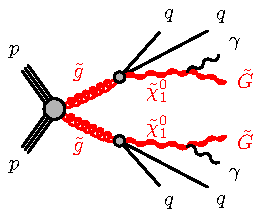
\includegraphics[width=0.45\textwidth]{gogo-qqqqphphGG-GMSB} ~~
%% %%     \includegraphics[width=0.45\textwidth]{C1C1-WWphphGG-GGM}
%% %%   \end{center}
%% %%   \caption{
%% %% Typical production and decay-chain processes for the gluino-production (left)
%% %%       and electroweak-production (right) instances of the
%% %%       GGM model for which the NLSP is a bino-like neutralino.
%% %% %      For the higgsino-bino models, the final
%% %% %      step of the cascade (the \neutralino decay) would have a
%% %% %      probability of order 50\% for producing a Higgs
%% %% %      (for the model with $\mu < 0$) or $Z$ (for the model with $\mu > 0$)
%% %% %      boson.
%% %%     \label{fig:feynman_bino}
%% %%   }
%% %% \end{figure}

%% %% \begin{figure}[tp]
%% %%   \begin{center}
%% %%     \includegraphics[width=0.45\textwidth]{gogo-qqqqbbphGG-h} ~~
%% %%     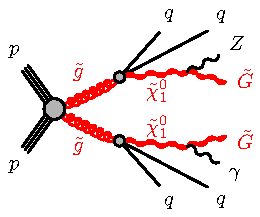
\includegraphics[width=0.45\textwidth]{gogo-qqqqphZGG-GMSB}
%% %%   \end{center}
%% %%   \caption{
%% %%     Typical production and decay-chain processes for the gluino-production
%% %%     and electroweak-production instances of the
%% %%     GGM model for which the NLSP is a higgsino-bino neutralino admixture.
%% %%     For the model with $\mu < 0$ (left), the final
%% %%     step of the cascade (the \neutralino decay) would have a
%% %%     probability of order 50\% of producing a Higgs boson rather than a
%% %%     photon or $Z$ boson; for the model
%% %%     with $\mu > 0$ (right), the \neutralino decay would have a
%% %%     probability of order 50\% of producing a Z boson rather than a photon.
%% %%     \label{fig:feynman_higgsino_bino}
%% %%   }
%% %% \end{figure}

%% %% \begin{figure}[tp]
%% %%   \begin{center}
%% %%     \includegraphics[width=0.45\textwidth]{C1N1-phlvGG-W}
%% %%   \end{center}
%% %%   \caption{
%% %% Typical production and decay-chain processes for the wino-NLSP model.
%% %% In this model, the \neutralino is a pure \winon state, while the
%% %% \chargino are the two charged wino states.
%% %%     \label{fig:feynman_wino}
%% %%   }
%% %% \end{figure}

%% %% %Three
%% %% The higgsino-bino GGM models incorporate an NLSP composed of
%% %% a higgsino-bino admixture, as well as
%% %% %including `gluino-higgsino'%, `squark-higgsino'
%% %% %and `gluino-higgsino-jets' models that incorporate degenerate sets
%% %% a degenerate octet of gluinos %and squarks
%% %% identical in nature to those of the
%% %% gluino-bino model. % and squark-bino models, respectively.
%% %% For the first %two
%% %% of these models, which is the focus of the photon+b analysis,
%% %% the higgsino mass parameter $\mu$ is required to be negative, and the composition
%% %% of the NLSP is set by adjusting $\mu$ and the GGM U(1) mass parameter
%% %% $M_1$ so that a constant ratio of the branching fraction of $\neutralino \to h + \gravitino$
%% %% to that of $\neutralino \to \gamma + \gravitino$ is maintained at
%% %% approximately 1.7:1 over the full range of NLSP masses.
%% %% In the limit that $m_{\neutralino} \gg m_Z$, the NLSP
%% %% branching fractions to $h + \gravitino$, $\gamma + \gravitino$,
%% %% and $Z + \gravitino$ approach 56\%, 33\%, and 11\%, respectively.
%% %% The GGM SU(3) mass parameter $M_3$ bears a direct relation to the
%% %% gluino mass, and is taken to be a free parameter in this $\mu < 0$ higgsino-bino
%% %% model, with all squark states decoupled.
%% %% %For the squark-higgsino model, the gluino
%% %% %mass and the mass of the right-handed up-type squark are decoupled, with the
%% %% %remaining squark masses treated as a single free parameter. For both of these models,
%% %% The GGM SU(2) mass parameter $M_2$ is set to a value of 2.5 TeV.
%% %% Four other electroweak gaugino states typically lie
%% %% within 25 GeV of the \neutralino NLSP: the two lightest charginos \chargino, and two
%% %% additional neutralinos \neutralinotwo and \neutralinothree.
%% %% The pair production of gluinos or any of these four additional gaugino
%% %% states leads to decays to the \neutralino via
%% %% cascades involving SM particles.

%% %% For the second of the higgsino-bino models, which is
%% %% the focus of the photon+j analysis, the $\mu$ parameter is
%% %% chosen to be positive, which suppresses the $h + \gravitino$
%% %% decay mode of the higgsino. As for the models described above,
%% %% the NLSP mass is taken to be a free parameter.
%% %% The $M_1$ and $\mu$ parameters are adjusted so that the branching
%% %% fractions of the $\neutralino$ to $\gamma + \gravitino$, $Z + \gravitino$
%% %% and $h + \gravitino$ are maintained close to 50\%, 49\% and 1\% for
%% %% most values of the $\neutralino$ and gluino masses.
%% %% In this model, the production of gluino pairs can be followed
%% %% by decays to both a single photon and a hadronically-decaying $Z$ boson, producing
%% %% events with a single isolated high-energy photon accompanied
%% %% by two jets.
%% %% In the case that the gluino mass is substantially
%% %% larger than the $\neutralino$ mass, additional jets can
%% %% be produced in the cascade.
%% %% Three additional electroweak gaugino states
%% %% lie close in mass to the \neutralino, allowing for the
%% %% possibility of SUSY production through pairs of these
%% %% states. Such events tend to produce fewer jets than those that proceed through gluino production,
%% %% but in certain regions of the model space can provide a significant
%% %% contribution to data samples selected to isolate the photon-plus-jets
%% %% signature. As for the $\mu < 0$ higgsino-bino model, the value of $M_3$, which is directly
%% %% related to the gluino mass, is taken to be a free parameter, $M_2$ is
%% %% set to a value of 2.5 TeV, and all squark states are decoupled.
%% %% Typical production and decay-chain processes for the two models
%% %% for which the NLSP is a higgsino-bino admixture are shown in Fig.~\ref{fig:feynman_higgsino_bino}.


%% %% Finally, the wino-NLSP model, which is the focus of the photon+$\ell$ analysis,
%% %% incorporates a set of three degenerate wino-like
%% %% NLSPs. This set includes the neutral \winon, which as the lightest
%% %% neutral gaugino is also referred to as the \neutralino,
%% %% as well as the two charged wino states, which form the \chargino states.
%% %% Production proceeds
%% %% %either through pairs of colored sparticles or
%% %% through the direct production of pairs of NLSP states;
%% %% %In either case
%% %% %the decay procedes through two wino-like NLSPs, and as a result
%% %% such events usually contain at least one \winon NLSP. Although
%% %% the \winon couples preferentially to the $Z$ boson relative to
%% %% the photon, the \winon decays into a photon+gravitino final state with unit branching fraction
%% %% for wino mass below that of the $Z$ boson.
%% %% The \winon branching fraction to photon+gravitino approaches
%% %% $\sin^2 \theta_W$ for wino masses far above that of the $Z$ boson.
%% %% Leptons can be produced either through the decays of charged wino
%% %% states, or through the decays of $Z$ bosons that arise from \winon
%% %% decay, leading to a significant probability that the overall final state
%% %% will contain both a photon and a lepton. In this model,
%% %% %a common squark and guino mass is taken as a free parameter
%% %% %along with the wino NLSP mass scale;
%% %% a common wino mass scale is taken as a free parameter, with
%% %% all other GGM mass parameters set to a value of \unit[2.5]{TeV}, except the squark masses,
%% %% which are set to infinity.
%% %% A production and decay diagram typical for this model is shown in Fig.~\ref{fig:feynman_wino}.
%% %% %In all cases, the decay chain
%% %% %procedes through the wino-like NLSP states.


%% %% For all five models considered here, the mass of the gravitino is chosen so that
%% %% the NLSP decay length is never greater than 1 mm. This ensures that all
%% %% particles arising from the decay of the NLSP are prompt, and in particular that
%% %% that the relationship between the point and direction of impact
%% %% of photons from NLSP decay upon the face of the detector is
%% %% consistent with that of a prompt photon (a separate analysis~\cite{Aad:2014gfa}
%% %% searches for GGM models with a longer-lived bino-like NLSP, leading to signatures with non-prompt photons).
%% %% In addition, the ratio
%% %% $\tan \beta$ of the two SUSY Higgs-doublet vacuum-expectation values is set to a value of 1.5;
%% %% %for all but the higgsino-bino model with positive $\mu$ and the wino-NLSP model; for those models
%% %% %$\tan \beta$ is set to 1.5.
%% %% for all five models, the phenomenology relevant to this search is only
%% %% weakly dependent on the value of $\tan \beta$.

%% The scenarios considered in this analysis are the
%% %% ones with only one \gam\ %i.e. $\g Z$ and $\g h$,
%% %% plus two \gravino\ in the final state, in the case \ninoone\ is a bino-higgsino admixture (\Fig \ref{fig:GGM_diagrams} (left)). Further details on the signal models and benchmark points
%% %% considered in this study are given in \Sec \ref{sec:sig_samples}.

%% En a\~no recientes, el esfuerzo por formular GMSB de un modo model-independent has led
%% el desarrollo de general gauge mediation (GGM) \cite{Meade:2008wd,Buican:2008ws}.
%% GGM inlcuye un sector observable con todos los campos de MSSM, junto con un sector oculto
%% que contiene la fuente del rompimiento de SUSY. En GGM, no tiene porque haber una jerarquia
%% entre los estados de color y los de no color, y por lo tanto no hay ninguna restriccion teorica
%% en la masa de los estados de color, aumentando la posibilidad de descubir GGM con los primeros
%% datos del LHC.

Se han realizado muchas busquedas de estas signatures en Tevatron \cite{Abazov:2007ag,Buescher:2005he}
y el LHC \cite{Aad:2012zza,Aad:2012jva,Aad:2011kz,Aad2012519,leptonphoton7,Chatrchyan:2011wc,Chatrchyan:2011ah,tagkey2015503}.

Este trabajo describe la busqueda de eventos con un foton aislado muy energetico, jets y energia faltante
con todos los datos de las colisiones $pp$ a una energia de centro de masa de 8 TeV tomadas durante
el a\~no 2012 con el detector ATLAS en el LHC, correspondiente a una luminosidad total integrada de 20.3 \ifb.

Esta busqueda es complementaria a otras busquedas en ATLAS con estados finales con
\gam\gam+\etmiss \cite{Aad2012519,ATLAS-CONF-2014-001}, $\gam+e/\mu+\etmiss$ \cite{ATLAS-CONF-2012-144},
$\gam+b+\etmiss$ \cite{Aad:2012jva}, y $Z+\etmiss$ \cite{ATLAS-CONF-2012-152}. El otro gran experimento del
LHC, CMS, tambien ha realizado estudios similares \cite{CMS-PAS-SUS-12-018,CMS-PAS-SUS-14-004}, aunque solo
en el caso de estados de puro bino o puro wino.\todo{Check/update this}

\begin{figure}[h!]
  \centering
  \includegraphics[width=0.31\textwidth]{figures/GGM_diagram_yy}
  \includegraphics[width=0.31\textwidth]{figures/GGM_diagram_yh}
  \includegraphics[width=0.31\textwidth]{figures/GGM_diagram_yZ}
  \caption{General production diagrams for GGM photon final states.}
  \label{fig:GGM_diagrams}
\end{figure}







Neutralinos
